%share memory
\subsection{Shared Memory}
In der Grafikkarte ist der Zugriff auf den globalen Speicher langsamer als auf den On-Chip-Speicher.  Nach dem Beispiel in \cite{cudapg}  kann man mehrmals verwendete Daten zunächst in das shared Memory kopieren und dann für die entsprechenden Operationen benutzen.
In der Multiplikation Vollmatrix mal Vektor wird jedes Vektorelement mehrmals gebraucht.
Nach Untersuchungen wählen wir einen eindimensionalen Block der Größe 64
Jedes Vektorelement wird 8 mal bnutzt in einem Block, d.h. in jeder Block bearbeitet
8 zerlegte Vektormultiplikationen. Die Abb. \ref{sharememory}
zeigt die Laufzeitenunterschiede von unterschiedlicher Implementierungen.
Egebnisse der Messungen stellen in Tabelle\ref{tab_shared_memory}.
\begin{figure}[htbp]
%\centering
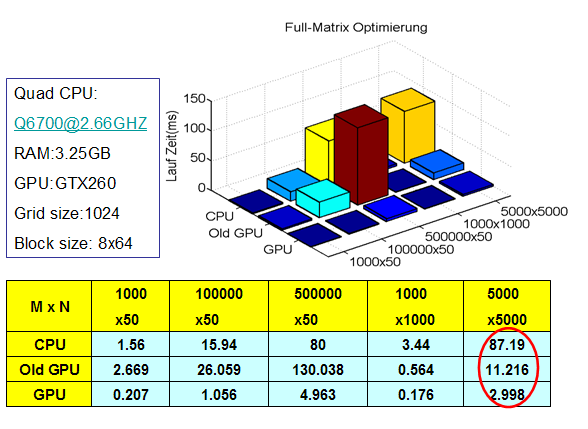
\includegraphics[width=3.5in]{../xby/pic/sharememory}
\caption{Vergleich von optimierte Vollmatrixmultiplikation mit C-Implementierung und nichtoptimierte GPU-Implementirung für $M$ * $N$ Vollmatrix}
\label{sharememory}
\end{figure}


%\usepackage{booktabs}
%\usepackage{tabularx}
\begin{table}
\renewcommand{\arraystretch}{1.3}
\caption{Ausführungszeiten der Vollmatrix-Vektormultipkation $ \bf{A_{mn} } \cdot \bf b$}
\label{tab_shared_memory}
%\begin{tabular}{|l|c|c|c|c|c|}
\centering
%\begin{tabular}{|p{46pt}p{28pt}p{30pt}p{28pt}p{30pt}p{30pt}|}
%\begin{tabularx}{350pt}{1xxxxx}
\begin{tabular}{|l||r|r|r|r|r|}

\hline
	$m$& $10^4$ & $10^5$ & 50000& $10^3 $ & 5000\\
    $n$& 50& 50& 50& $10^3$ & 5000 \\

\hline
\hline
CPU(ms)& 1.56&    15.94& 				80&      3.44& 87.9\\

old GPU/CPU& 1.711& 1.6348&   1.62548&  0.164&  0.12854\\

GPU/CPU & 0.133& 0.0662&     0.06204&   0.0512& 0.03438\\


\hline
\end{tabular}
%\end{tabularx}
\end{table}
Die optimierte GPU-Implementierung ist immer schnelle als die CPU-Implementierung  und die nichtoptimierte Version. Für eine Matrixgröße 5000x5000 kann läuft das CUDA-Programm 30 mal schneller als die CPU-Implementierung.

